\documentclass[a4paper,twoside,openright,makeidx,12pt]{book}
%\usepackage{draftcopy}
%%$Id: macro.tex,v 1.10 2004/12/08 13:38:58 acary Exp $


%\usepackage{a4wide}
\textheight 25cm
\textwidth 16.5cm
\topmargin -1cm
%\evensidemargin 0cm
\oddsidemargin 0cm
\evensidemargin0cm
\usepackage{layout}


\usepackage{amsmath}
\usepackage{amssymb}
\usepackage{minitoc}
%\usepackage{glosstex}
\usepackage{colortbl}
\usepackage{hhline}
\usepackage{longtable}

%\usepackage{glosstex}
%\def\glossaryname{Glossary of Notation}
\def\listacronymname{Acronyms}

\usepackage[outerbars]{changebar}\setcounter{changebargrey}{20}
%\glxitemorderdefault{acr}{l}

%\usepackage{color}
\usepackage{graphicx,epsfig}
\graphicspath{{./Figures/}}
\usepackage[T1]{fontenc}
\usepackage{rotating}

%\usepackage{algorithmic}
%\usepackage{algorithm}
\usepackage{ntheorem}
\usepackage{natbib}


%\renewcommand{\baselinestretch}{2.0}
\setcounter{tocdepth}{2}     % Dans la table des matieres
\setcounter{secnumdepth}{3}  % Avec un numero.



\newtheorem{definition}{Definition}
\newtheorem{lemma}{Lemma}
\newtheorem{claim}{Claim}
\newtheorem{remark}{Remark}
\newtheorem{assumption}{Assumption}
\newtheorem{example}{Example}
\newtheorem{conjecture}{Conjecture}
\newtheorem{corollary}{Corollary}
\newtheorem{OP}{OP}
\newtheorem{problem}{Problem}
\newtheorem{theorem}{Theorem}


\newcommand{\CC}{\mbox{\rm $~\vrule height6.6pt width0.5pt depth0.25pt\!\!$C}}
\newcommand{\ZZ}{\mbox{\rm \lower0.3pt\hbox{$\angle\!\!\!$}Z}}
\newcommand{\RR}{\mbox{\rm $I\!\!R$}}
\newcommand{\HH}{\mbox{\rm $I\!\!H$}}
\newcommand{\NN}{\mbox{\rm $I\!\!N$}}

\newcommand{\Mnn}{\mathcal M^{n\times n}}
\newcommand{\Mnp}[2]{\ensuremath{\mathcal M^{#1\times #2}}}



\newcommand{\Frac}[2]{\displaystyle \frac{#1}{#2}}

\newcommand{\DP}[2]{\displaystyle \frac{\partial {#1}}{\partial {#2}}}

% c++ variables writting
\newcommand{\varcpp}[1]{\textit{#1}}
% itemize
\newcommand{\bei}{\begin{itemize}}
\newcommand{\ei}{\end{itemize}}

\newcommand{\ie}{i.e.}
\newcommand{\eg}{e.g.}
\newcommand{\cf}{c.f.}
\newcommand{\putidx}[1]{\index{#1}\textit{#1}}

\def\Er{{\rm I\! R}}
\def\En{{\rm I\! N}} 
\def\Ec{{\rm I\! C}}
 
\def\zc{\hat{z}}
\def\wc{\hat{w}}

\font\tete=cmr8 at 8 pt


% normal tangent
\def\n{{\hbox{\tiny{N}}}}
\def\t{{\hbox{\tiny{T}}}}
\def\nt{\hbox{\tiny{NT}}}
\def\nsf{\hbox{\tiny{\textsf N}}}
\def\tsf{\hbox{\tiny{\textsf T}}}
\def\sigman{\sigma_{\n}}
\def\sigmat{\sigma_{\t}}
\def\sigmant{\sigma_{\nt}}
\def\epsn{\epsilon_{\n}}
\def\epst{\epsilon_{\t}}
\def\epsnt{\epsilon_{\nt}}
\def\eps{\epsilon}
\def\veps{\varepsilon}
\def\sig{\sigma}
\def\Rn{R_{\n}}
\def\Rt{R_{\t}}
\def\cn{c_{\n}}
\def\Cn{C_{\n}}
\def\ct{c_{\t}}
\def\Ct{C_{\t}}
\def\un{u_{\n}}
\def\ut{\buu_{\t}}
\def\uut{u_{\t}}
\def\unc{u_{\n}^c}
\def\utc{\buu_{\t}^c}
\def\vn{v_{\n}}
\def\vt{v_{\t}}
\def\rr{\hbox{\tiny{\textsf R}}}
\def\irr{\hbox{\tiny{\textsf{IR}}}}
\def\rn{r_{\n}}
\def\rt{\brr_{\t}}
\def\rnc{r_{\n}^c}
\def\rtc{\brr_{\t}^c}
\def\trn{\Tilde{r}_{\n}}
\def\trt{\Tilde{\brr}_{\t}}
\def\tr{\Tilde{\brr}}
\def\tv{\Tilde{\bvv}}
\def\vn{v_{\n}}
\def\vt{\bvv_{\t}}
\def\adh{\mathsf{adh}}
\def\adj{\hbox{\tiny{\textsf{adj}}}}
\def\adjc{\hbox{\tiny{\textsf{adjC}}}}
\def\adja{\hbox{\tiny{\textsf{adjA}}}}
\def\cc{\hbox{\tiny{\textsf C}}}
\def\ca{\hbox{\tiny{\textsf A}}}

\DeclareMathOperator{\proj}{proj}
\DeclareMathOperator{\expm}{expm}
\DeclareMathOperator{\dexp}{dexp}
\DeclareMathOperator{\dlexp}{d^l exp}
\DeclareMathOperator{\drexp}{d^r exp}
\DeclareMathOperator{\dexpm}{dexpm}
\DeclareMathOperator{\expq}{expq}
\DeclareMathOperator{\dexpq}{dexpq}
\DeclareMathOperator{\Ad}{Ad}
\DeclareMathOperator{\ad}{ad}
\DeclareMathOperator{\dd}{d}



%%  Les ensembles de nombres  C. Fiorio (fiorioÊatÊmath.tu-berlin.de) 
%
\def\nbR{\ensuremath{\mathrm{I\!R}}} % IR
\def\nbN{\ensuremath{\mathrm{I\!N}}} % IN
\def\nbF{\ensuremath{\mathrm{I\!F}}} % IF
\def\nbH{\ensuremath{\mathrm{I\!H}}} % IH
\def\nbK{\ensuremath{\mathrm{I\!K}}} % IK
\def\nbL{\ensuremath{\mathrm{I\!L}}} % IL
\def\nbM{\ensuremath{\mathrm{I\!M}}} % IM
\def\nbP{\ensuremath{\mathrm{I\!P}}} % IP

%----------------------------------------------------------------------
%                  Modification des subsubsections
%----------------------------------------------------------------------
\makeatletter
\renewcommand\thesubsubsection{\thesubsection.\@alph\c@subsubsection}
\makeatother

%----------------------------------------------------------------------
%             Redaction note environnement
%----------------------------------------------------------------------
\makeatletter
\theoremheaderfont{\scshape}
\theoremstyle{marginbreak}
\theorembodyfont{\upshape}
%\newtheorem{rque}{\bf Remarque}[chapter]
%\newtheorem{rque1}{\bf \fsc{Remarque}}[chapter] !!! \fsc est une commande french
\newtheorem{ndr1}{\textbf{\textsc{Redaction note}}}[section]

\newenvironment{ndr}%
{%
\tt
%\centerline{---oOo---}
\noindent\begin{ndr1}%
}%
{%
\begin{flushright}%
%\vspace{-1.5em}\ding{111}
\end{flushright}%
\end{ndr1}%
%\centerline{---oOo---}
}

\makeatother

%----------------------------------------------------------------------
%             Redaction note environnement V.ACARY
%----------------------------------------------------------------------
\makeatletter
\theoremheaderfont{\scshape}
\theoremstyle{marginbreak}
\theorembodyfont{\upshape}
%\newtheorem{rque}{\bf Remarque}[chapter]
%\newtheorem{rque1}{\bf \fsc{Remarque}}[chapter] !!! \fsc est une commande french
\newtheorem{ndr1va}{\textbf{\textsc{Redaction note V. ACARY}}}[section]

\newenvironment{ndrva}%
{%
\tt
%\centerline{---oOo---}
\noindent\begin{ndr1va}%
}%
{%
\begin{flushright}%
%\vspace{-1.5em}\ding{111}
\end{flushright}%
\end{ndr1va}%
%\centerline{---oOo---}
}

\makeatother
%----------------------------------------------------------------------
%             Redaction note environnement V.ACARY
%----------------------------------------------------------------------
\makeatletter
\theoremheaderfont{\scshape}
\theoremstyle{marginbreak}
\theorembodyfont{\upshape}
%\newtheorem{rque}{\bf Remarque}[chapter]
%\newtheorem{rque1}{\bf \fsc{Remarque}}[chapter] !!! \fsc est une commande french
\newtheorem{ndr1fp}{\textbf{\textsc{Redaction note F. PERIGNON}}}[section]

\newenvironment{ndrfp}%
{%
\tt
%\centerline{---oOo---}
\noindent\begin{ndr1fp}%
}%
{%
\begin{flushright}%
%\vspace{-1.5em}\ding{111}
\end{flushright}%
\end{ndr1fp}%
%\centerline{---oOo---}
}

\makeatother
%----------------------------------------------------------------------
%                  Chapter head enviroment
%----------------------------------------------------------------------
\newenvironment{chapter_head}
{%
\begin{center}%
-------------------- oOo --------------------\\%
\ \\%
\begin{minipage}[]{14cm}%
\noindent\normalsize\advance\baselineskip-1pt %
}%
{%
\par\end{minipage}%
\ \\%
\ \\%
-------------------- oOo --------------------
\end{center}%
\vspace*{\stretch{1}}%
\clearpage%
\thispagestyle{empty}%
\vspace*{\stretch{1}}%
\minitoc%
\vspace*{\stretch{2}}%
\clearpage%
}


\newcommand{\contract}{{\,:\,}}

%%% Local Variables: 
%%% mode: latex
%%% TeX-master: "report"
%%% End: 

%$Id: macro.tex,v 1.10 2004/12/08 13:38:58 acary Exp $


%\usepackage{a4wide}
\textheight 25cm
\textwidth 16.5cm
\topmargin -1cm
%\evensidemargin 0cm
\oddsidemargin 0cm
\evensidemargin0cm
\usepackage{layout}


\usepackage{amsmath}
\usepackage{amssymb}
\usepackage{minitoc}
%\usepackage{glosstex}
\usepackage{colortbl}
\usepackage{hhline}
\usepackage{longtable}

%\usepackage{glosstex}
%\def\glossaryname{Glossary of Notation}
\def\listacronymname{Acronyms}

\usepackage[outerbars]{changebar}\setcounter{changebargrey}{20}
%\glxitemorderdefault{acr}{l}

%\usepackage{color}
\usepackage{graphicx,epsfig}
\graphicspath{{./Figures/}}
\usepackage[T1]{fontenc}
\usepackage{rotating}

%\usepackage{algorithmic}
%\usepackage{algorithm}
\usepackage{ntheorem}
\usepackage{natbib}


%\renewcommand{\baselinestretch}{2.0}
\setcounter{tocdepth}{2}     % Dans la table des matieres
\setcounter{secnumdepth}{3}  % Avec un numero.



\newtheorem{definition}{Definition}
\newtheorem{lemma}{Lemma}
\newtheorem{claim}{Claim}
\newtheorem{remark}{Remark}
\newtheorem{assumption}{Assumption}
\newtheorem{example}{Example}
\newtheorem{conjecture}{Conjecture}
\newtheorem{corollary}{Corollary}
\newtheorem{OP}{OP}
\newtheorem{problem}{Problem}
\newtheorem{theorem}{Theorem}


\newcommand{\CC}{\mbox{\rm $~\vrule height6.6pt width0.5pt depth0.25pt\!\!$C}}
\newcommand{\ZZ}{\mbox{\rm \lower0.3pt\hbox{$\angle\!\!\!$}Z}}
\newcommand{\RR}{\mbox{\rm $I\!\!R$}}
\newcommand{\HH}{\mbox{\rm $I\!\!H$}}
\newcommand{\NN}{\mbox{\rm $I\!\!N$}}

\newcommand{\Mnn}{\mathcal M^{n\times n}}
\newcommand{\Mnp}[2]{\ensuremath{\mathcal M^{#1\times #2}}}



\newcommand{\Frac}[2]{\displaystyle \frac{#1}{#2}}

\newcommand{\DP}[2]{\displaystyle \frac{\partial {#1}}{\partial {#2}}}

% c++ variables writting
\newcommand{\varcpp}[1]{\textit{#1}}
% itemize
\newcommand{\bei}{\begin{itemize}}
\newcommand{\ei}{\end{itemize}}

\newcommand{\ie}{i.e.}
\newcommand{\eg}{e.g.}
\newcommand{\cf}{c.f.}
\newcommand{\putidx}[1]{\index{#1}\textit{#1}}

\def\Er{{\rm I\! R}}
\def\En{{\rm I\! N}} 
\def\Ec{{\rm I\! C}}
 
\def\zc{\hat{z}}
\def\wc{\hat{w}}

\font\tete=cmr8 at 8 pt


% normal tangent
\def\n{{\hbox{\tiny{N}}}}
\def\t{{\hbox{\tiny{T}}}}
\def\nt{\hbox{\tiny{NT}}}
\def\nsf{\hbox{\tiny{\textsf N}}}
\def\tsf{\hbox{\tiny{\textsf T}}}
\def\sigman{\sigma_{\n}}
\def\sigmat{\sigma_{\t}}
\def\sigmant{\sigma_{\nt}}
\def\epsn{\epsilon_{\n}}
\def\epst{\epsilon_{\t}}
\def\epsnt{\epsilon_{\nt}}
\def\eps{\epsilon}
\def\veps{\varepsilon}
\def\sig{\sigma}
\def\Rn{R_{\n}}
\def\Rt{R_{\t}}
\def\cn{c_{\n}}
\def\Cn{C_{\n}}
\def\ct{c_{\t}}
\def\Ct{C_{\t}}
\def\un{u_{\n}}
\def\ut{\buu_{\t}}
\def\uut{u_{\t}}
\def\unc{u_{\n}^c}
\def\utc{\buu_{\t}^c}
\def\vn{v_{\n}}
\def\vt{v_{\t}}
\def\rr{\hbox{\tiny{\textsf R}}}
\def\irr{\hbox{\tiny{\textsf{IR}}}}
\def\rn{r_{\n}}
\def\rt{\brr_{\t}}
\def\rnc{r_{\n}^c}
\def\rtc{\brr_{\t}^c}
\def\trn{\Tilde{r}_{\n}}
\def\trt{\Tilde{\brr}_{\t}}
\def\tr{\Tilde{\brr}}
\def\tv{\Tilde{\bvv}}
\def\vn{v_{\n}}
\def\vt{\bvv_{\t}}
\def\adh{\mathsf{adh}}
\def\adj{\hbox{\tiny{\textsf{adj}}}}
\def\adjc{\hbox{\tiny{\textsf{adjC}}}}
\def\adja{\hbox{\tiny{\textsf{adjA}}}}
\def\cc{\hbox{\tiny{\textsf C}}}
\def\ca{\hbox{\tiny{\textsf A}}}

\DeclareMathOperator{\proj}{proj}
\DeclareMathOperator{\expm}{expm}
\DeclareMathOperator{\dexp}{dexp}
\DeclareMathOperator{\dlexp}{d^l exp}
\DeclareMathOperator{\drexp}{d^r exp}
\DeclareMathOperator{\dexpm}{dexpm}
\DeclareMathOperator{\expq}{expq}
\DeclareMathOperator{\dexpq}{dexpq}
\DeclareMathOperator{\Ad}{Ad}
\DeclareMathOperator{\ad}{ad}
\DeclareMathOperator{\dd}{d}



%%  Les ensembles de nombres  C. Fiorio (fiorioÊatÊmath.tu-berlin.de) 
%
\def\nbR{\ensuremath{\mathrm{I\!R}}} % IR
\def\nbN{\ensuremath{\mathrm{I\!N}}} % IN
\def\nbF{\ensuremath{\mathrm{I\!F}}} % IF
\def\nbH{\ensuremath{\mathrm{I\!H}}} % IH
\def\nbK{\ensuremath{\mathrm{I\!K}}} % IK
\def\nbL{\ensuremath{\mathrm{I\!L}}} % IL
\def\nbM{\ensuremath{\mathrm{I\!M}}} % IM
\def\nbP{\ensuremath{\mathrm{I\!P}}} % IP

%----------------------------------------------------------------------
%                  Modification des subsubsections
%----------------------------------------------------------------------
\makeatletter
\renewcommand\thesubsubsection{\thesubsection.\@alph\c@subsubsection}
\makeatother

%----------------------------------------------------------------------
%             Redaction note environnement
%----------------------------------------------------------------------
\makeatletter
\theoremheaderfont{\scshape}
\theoremstyle{marginbreak}
\theorembodyfont{\upshape}
%\newtheorem{rque}{\bf Remarque}[chapter]
%\newtheorem{rque1}{\bf \fsc{Remarque}}[chapter] !!! \fsc est une commande french
\newtheorem{ndr1}{\textbf{\textsc{Redaction note}}}[section]

\newenvironment{ndr}%
{%
\tt
%\centerline{---oOo---}
\noindent\begin{ndr1}%
}%
{%
\begin{flushright}%
%\vspace{-1.5em}\ding{111}
\end{flushright}%
\end{ndr1}%
%\centerline{---oOo---}
}

\makeatother

%----------------------------------------------------------------------
%             Redaction note environnement V.ACARY
%----------------------------------------------------------------------
\makeatletter
\theoremheaderfont{\scshape}
\theoremstyle{marginbreak}
\theorembodyfont{\upshape}
%\newtheorem{rque}{\bf Remarque}[chapter]
%\newtheorem{rque1}{\bf \fsc{Remarque}}[chapter] !!! \fsc est une commande french
\newtheorem{ndr1va}{\textbf{\textsc{Redaction note V. ACARY}}}[section]

\newenvironment{ndrva}%
{%
\tt
%\centerline{---oOo---}
\noindent\begin{ndr1va}%
}%
{%
\begin{flushright}%
%\vspace{-1.5em}\ding{111}
\end{flushright}%
\end{ndr1va}%
%\centerline{---oOo---}
}

\makeatother
%----------------------------------------------------------------------
%             Redaction note environnement V.ACARY
%----------------------------------------------------------------------
\makeatletter
\theoremheaderfont{\scshape}
\theoremstyle{marginbreak}
\theorembodyfont{\upshape}
%\newtheorem{rque}{\bf Remarque}[chapter]
%\newtheorem{rque1}{\bf \fsc{Remarque}}[chapter] !!! \fsc est une commande french
\newtheorem{ndr1fp}{\textbf{\textsc{Redaction note F. PERIGNON}}}[section]

\newenvironment{ndrfp}%
{%
\tt
%\centerline{---oOo---}
\noindent\begin{ndr1fp}%
}%
{%
\begin{flushright}%
%\vspace{-1.5em}\ding{111}
\end{flushright}%
\end{ndr1fp}%
%\centerline{---oOo---}
}

\makeatother
%----------------------------------------------------------------------
%                  Chapter head enviroment
%----------------------------------------------------------------------
\newenvironment{chapter_head}
{%
\begin{center}%
-------------------- oOo --------------------\\%
\ \\%
\begin{minipage}[]{14cm}%
\noindent\normalsize\advance\baselineskip-1pt %
}%
{%
\par\end{minipage}%
\ \\%
\ \\%
-------------------- oOo --------------------
\end{center}%
\vspace*{\stretch{1}}%
\clearpage%
\thispagestyle{empty}%
\vspace*{\stretch{1}}%
\minitoc%
\vspace*{\stretch{2}}%
\clearpage%
}


\newcommand{\contract}{{\,:\,}}

%%% Local Variables: 
%%% mode: latex
%%% TeX-master: "report"
%%% End: 

\usepackage{pifont}
 \usepackage{lscape}



\includeonly{}
\usepackage{fancyheadings} 
\usepackage{verbatim}

% package pour les images des use cases
%\usepackage[dvips]{graphicx}

\pagestyle{fancy} 
\renewcommand{\chaptermark}[1]% 
{\markboth{{Chap-- \thechapter.\ #1}}{}} 
\renewcommand{\sectionmark}[1]% 
{\markright{{\thesection.\ #1}}} 
\setlength{\headrulewidth}{0.5pt} 
\setlength{\footrulewidth}{0.5pt} 
\newcommand{\helv}{% 
\fontfamily{phv}\fontseries{b}\fontsize{9}{11}\selectfont} 
\lhead[\helv \thepage]{\helv \rightmark} 
\rhead[\helv \leftmark]{\helv \thepage} 
\cfoot{Software Specification Document -- November 25, 2004}

\makeindex

\begin{document}
\pagestyle{empty}
\renewcommand{\arraystretch}{1.8}

\input{coverSSD.tex}

\tableofcontents


\pagestyle{fancy}
%---------------------------------------------------------------------%
\cleardoublepage

\pagenumbering{arabic}
\chapter{Introduction}
\label{Sec:SSD-Intoduction}
\section{Purpose of this document}
\label{Sec:SSD-Purpose-Scope}
The purpose of the Software Specification Document Document is to define the user and software requirements, and the architecture design of \ac{siconos}/Numerics.
The \ac{ssd} is a contractual document which aims to define precisely the software to realize. It describes functionalities and characteristics of the product and constraints of development and exploitation. It is addressed to users and software framework builders. \\
\\
This document will be used as basis : 
\begin{itemize}
\item For the evaluation of the final product,
\item For the editing of test plan,
\item For the editing of the \ac{ddd}.
\end{itemize}


\section{Context of \ac{numerics}}
\label{Sec:SSD-Context}
\ac{numerics} is toolbox for computation relating to non-smooth dynamical systems. The main use of its capabilities is in the \ac{siconos} platform.

%\subsection{Exploitation context}


\section{References}
\label{Sec:SSD-References}
\begin{itemize}
\item \textbf{"Guide to applying the software engineering standards to small software projects", BSSC(96)2 Issue1, ESA 1996}
\item \ac{tm}
\item \ac{SICONOS} Contract Number IST-2001-37172 and annexes

\end{itemize}




\section{Overview}
This software specification is composed of two phases :
\begin{enumerate}
\item The specification of the requirements
	\begin{itemize}
	\item A general description of the project. This part explains the purpose of this project and its integration into European project \ac{SICONOS}.
	\item The problem definition phase. The scope of the software must be defined. Specific user requirements must be identified and documented. The section has to provide a general description of what the user expects the software to do. It should state the specific user requirements as clearly and consistently as possible. 
	\end{itemize}
\item The architecture design\\
	It defines and describes the design of the system, in a manner that allows to elaborate it in details progressively. 
\end{enumerate}




%---------------------------------------------------------------------%
\newpage
\chapter{General Description}
\label{Sec:SSD-GeneralDescription}
%$Id: GeneralDescription.tex,v 1.32 2004/12/17 10:26:15 charlety Exp $
\section{Relation to the \ac{SICONOS} project}
\ac{SICONOS} is the European Project  IST2001-37172, funded by the Commission of the European Communities, from September 1, 2002, to August 31, 2006.
It is a project of the Information Society Technologies programme, fifth framework programme (FP5). This project's goal is the study of complementarity dynamical systems (a class of hybrid dynamical systems).


It gathers scientists from various communities : Mechanics, Applied Mathematics, Systems and Control, and Numerical Analysis and from various European countries : United Kingdom, Netherlands, Italy, Switzerland, Spain and France. 

The name \ac{SICONOS} comes from the title of the project : Modelling, Simulation and Control of Non-smooth Dynamical Systems. 

For example, a Non Smooth Dynamical System could be a system that incorporates friction and/or impacts for a mechanical one, or switchings for an electrical one. 

The strategic aim of this project is the development of novel algorithms and numerical routines for the qualitative analysis, simulation and feedback control of non-smooth complementarity dynamical systems. The output of \ac{SICONOS} will be an integrated numerical software package for the virtual prototyping of systems with discontinuities and development of novel control techniques for this class of dynamical systems. Therefore, this project is clearly focused on the development over 4 years of a user-friendly, versatile and computationally effective numerical tool for non-smooth systems, validated through its application to 3 key engineering problems : power electronic converters, walking robots and automotive systems. 

This project is divided into 7 work-packages :
\begin{itemize}
\item WP1 - Mathematical Analysis.
\item WP2 - Numerical Methods/Software Implementation. 
\item WP3 - Modelling.
\item WP4 - Bifurcation Analysis.
\item WP5 - Stabilization of trajectories and control related issues.
\item WP6 - Applications, Proof of Concept and Integration.
\item WP7 - Project Management, Dissemination and Exploitation of Results.
\end{itemize}

\ac{lmgc}, \ac{inria} and more particularly BIPOP team, are involved in WP2. Originally, the objectives of the Work Package 2 were defined in the Annex 2 of the project as follows :
\begin{enumerate}
\item Development of numerical methods for:     
        \begin{itemize}
        \item robust zero-crossing detection.
        \item time integration of complementarity systems.
        \item solution continuation and bifurcation detection for complementarity problems.
        \item Control design and validation.
        \end{itemize}
\item Designing an object-oriented algorithm structure to get:
        \begin{itemize}
        \item sufficient flexibility and potential incorporation of various classes of systems.
        \item real-time constraints for virtual reality applications.
        \item openness for easy insertion of new modules.
        \item link with other control applications.
        \end{itemize}
\end{enumerate}


%As part of our training course, we have to design and develop the basis of the SICONOS software platform.

\section{Relation to predecessor and successor projects}

The goal of this project is not redeveloping existing numerical routines, but providing framework for non-smooth problems. Particularly we want to reuse :
  \begin{itemize}
    \item Existing numerical tools dedicated to non smooth systems (\ac{lmgc90},\ldots ).
    \item Existing description tools for specific complex applications (\ac{modelica}, \ac{simulink}, \ac{scicos}, \ldots).
    \item Existing modelling softwares for standard dynamical systems (\textsf{Auto}\textsuperscript{\copyright},\ldots).
  \end{itemize}

Especially, we will use \ac{scilab}, numerical libraries (LAPACK, ...) and modules of \ac{lmgc90}. 


\subsection{Predecessor project : \ac{lmgc90}}


 \ac{lmgc90} is an existing platform for modelling interaction problems developed in FORTRAN90 in \ac{lmgc}. This software is made of a  library of components (F90 modules) which can be used through a macro-language named \ac{chic}). For the  basic algebra computations, this software relies on public numerical libraries such as LAPACK95, LAPACK and  BLAS. 

Although this software was designed in an oriented object way, one drawback is that Fortran 90 is not a real object-oriented language (lack of inheritance, template programming, dynamic polymorphism, \ldots ).  Indeed, it could be difficult to add new modules and maintain the code. 

%% \subsection{Evolution of the  SICONOS platform}
%% Three functionalities of the platform will be developed after first version of SICONOS software : 
%% \begin{itemize} 
%% \item SICONOS/Analysis : Analysis of solution.
%% \item SICONOS/Control : Control design and validation.
%% \item SICONOS/pre-post : Pre- and Post-Processing.
%% \end{itemize}

\section{Function and purpose}





The \ac{siconos} software is dedicated to the Modelling, Simulation, Analysis and Control of non smooth dynamical systems, i.e., abstract evolution problem where the non smooth character is crucial. To put it more  precisely, six major sets of functionalities have been identified :
\begin{enumerate}
\item Low level numerical tools {\acs{numerics}} \\
\ac{numerics} is dedicated to the computation of basic well-identified problems (linear algebra, mathematical programming, ...). Besides dedicated development for Non Smooth dynamical systems it should call external libraries for scientific computing. Furthermore, this module should be encapsulated for standalone \ac{xxxlab} use (see \ref{Sec:SICONOS/Numerics}).

\item Modelling and Simulation tools. {\acs{kernel}} \\
  \ac{kernel} of the software is dedicated to the modelling and the simulation of  the \ac{nsds}. For the modelling part, several canonical model, relevant from a numerical point of view will be defined for the dynamics of the system such as IVP and BVP coupled with a non smooth law (LCP, NCP, QP, AVI, ...). For the simulation part, robust time-integration method (Event driven, Time-stepping, ..) of the dynamics  and numerical solvers for non smooth laws  will be implemented. This module will only work on formalized models, i.e. canonical well identified models which represent the general abstract classes of \ac{nsds} (see the \ac{SICONOS} Theory Manual \textsf{\ac{siconos}/TM}). This module is the core of the software (see \ref{Sec:SICONOS/Engine}).

\item Front End interface. {\acs{frontend}} \\
  The goal of \ac{frontend} is to allow the users to implement  numerical resolution strategies and to drive numerical algorithms. It should be used through a driving interface based on a object oriented scriptiong language or through standard scientific computing software such as \ac{matlab} or \ac{scilab} (see \ref{Sec:SICONOS/Front-End}). 

\item Analysis tools. {\acs{analysis}} \\
\ac{analysis} must be able to characterize the existence and stability of solution. Efficient methods and algorithms for the parametric continuation of solutions and identification of bifurcation are also needed %(see \ref{Sec:SICONOS/Analysis}).


\item Control tools. {\acs{control}} \\
\ac{control} is for the design and the validation of control strategies for non smooth systems. This will contain standard functionalities of Control such as Feedback control with observers, trajectory planning, Optimal Control with state and control constraints, etc.%(see \ref{Sec:SICONOS/Control}).

\item {\acs{imse}}\\
 \ac{imse} provides a  modelling and visualization environment for the \ac{siconos}/Engine %(see \ref{Sec:SICONOS/pre-post}).
\end{enumerate}



\section{Environmental considerations}


The development of the software has to take into account the diversity of users. For each types of users, several constraints in terms of development has to be taken into account :
\begin{itemize}
\item End users %(see \ref{Sec:End-user}). 
For this type of users, user-friendly and interactive graphical interface are needed. This is the goal of the Front-End which must be integrated in a classical software for scientific computing as \ac{matlab} or \ac{scilab}.

\item Numerical routines developers %(see \ref{Sec:Expert-user}). 
For this type of users, the software we plan to develop should be modular and easy to extend with additional numerical routines.   Particularly for this of users, the Front End must be able to call every methods in the platform (and not just higher-level method) in order to validate promptly the new algorithm inserted.

\item Frame work builders %(see \ref{Sec:Developer}). 
For this type of users, the architecture must be modular and well documented in order to be maintained and modified easily. To reach this goal,  standard methods of Object Oriented Analysis and Design must be used.
\end{itemize}

The target system on hardware and operating system will be :
\begin{itemize}
\item PC/Linux
\item PC/Windows
\item Sun Workstation/Suns-Solaris
\item Apple/Mac OS X
\end{itemize}
More precision is given in the section "portability requirements", in chapter 3.


\section{Relation to other systems}
Three types of systems may be in relation with the \ac{siconos} platform.


\subsection{Existing modelling softwares}



Due to the fact that the \ac{siconos}/Engine is only devoted to grasp problems which are already formalized, a standalone  use of the software needs only to provide a formalized model. Otherwise, to treat plain, complex physical problem, the software should use some specific plug-ins. These plug-ins may be, for instance, interfaced  existing modelling softwares.     


The existing modelling software must be used for the description and the modelling of physical process. The first reason is the habits of the various community in using such software and the second is that this is not possible in term of development cost to re-implement such systems. Several systems for each scientific fields will be interfaced with the platform %using standard protocol as CORBA for Object Oriented modelling tool and 
dynamic linking or \ac{matlab} / \ac{scilab} functions.



To fulfil the constraints to re-use the existing development and software, the product must implement this two functionalities :
\begin{itemize}
\item To have a user plug-in interface to use in an easy way the code which already model, non smooth dynamical. This users plug-in system intend to provide to the user the possibility to input his data without recompiling the platform
\item To have a expert plug-in system, which allows us to specify the behaviour of a generic type of \ac{nsds} in the platform by loading dynamically new types of derived systems.
\end{itemize}

\subsection{Existing numerical routines and libraries}

 A lot of standard numerical libraries are already used to do standard computations in algebra (BLAS/LAPACK), numerical integration (Numerical recipes, LSODAR), numerical optimization. This standard tools are generally developed in C or Fortran 77 for efficiency constraints. The platform must be able to interface with such libraries.
\subsection{Existing front-end and interface to scientific computing software.}
Existing front-end and interface to scientific computing software. Finally, the platform has to be interfaced with the standard scientific computing software (\ac{matlab}, \ac{scilab}, ...) and standard computer Algebra System (CAS) (Maple, Mathematica, Ginac, ...) 



\section{General constraints}

The following general constraints on software design have to be taken into account :
\begin{itemize}
\item Use of Object Oriented analysis and design, to ensure software quality attributes and to allow modern software technologies. The platform aims to factorize existing methods for solving non smooth systems and provide a common framework for new development.  It requires that the architecture must be developed with Object oriented Language. In order to facilitate the interface with low-level languages (C, F77, see below) the choice of C++ seems to be more relevant.
\item Use of low level languages for numerical efficiency and parallelization in \ac{siconos}/Numerics. The application which are addressed requires computational efficiency in particular for large systems (for example in mechanics) or for real time applications. 
%\item Use of CORBA protocol for integration and interfaces, in order to : be platform independent, be robust, allow multiple languages and multiple environments, integrate existing developments.  The interface with existing modelling softwares must be platform independent. 
\item Use of \ac{xml} technology for data representation.
\end{itemize}

\newpage
\section{Model description}
In this section we present more precisely the six major functionalities of the \ac{siconos} software. In this section the relation between the functionalities are explicitly stated.

\subsection{The six majors functionalities}

The six major functionalities of the platform are recalled in the Table~\ref{Tab:SICONOS-func} and are depicted on the Figure~\ref{Fig:SICONOS-func}. 

\begin{table}[htbp]
  \centering
  \begin{tabular}[c]{|l|l|}
\hline
Name of the module & Functionality\\
\hline\hline
\ac{numerics}  & Low level numerical tools \\\hline
\ac{kernel} & Modelling and numerical simulation \\\hline
 \ac{frontend} & Command interactive user interface\\\hline
 \ac{analysis}  & Analysis of solution\\\hline
 \ac{control}  & Control design and validation\\\hline
 \ac{imse}  & Integrated modeling and Simulation Environment\\
\hline
  \end{tabular}
  \caption{The six major functionalities of the \ac{siconos} Platform}
  \label{Tab:SICONOS-func}
\end{table}

\begin{figure*}[htbp]
  \centering
  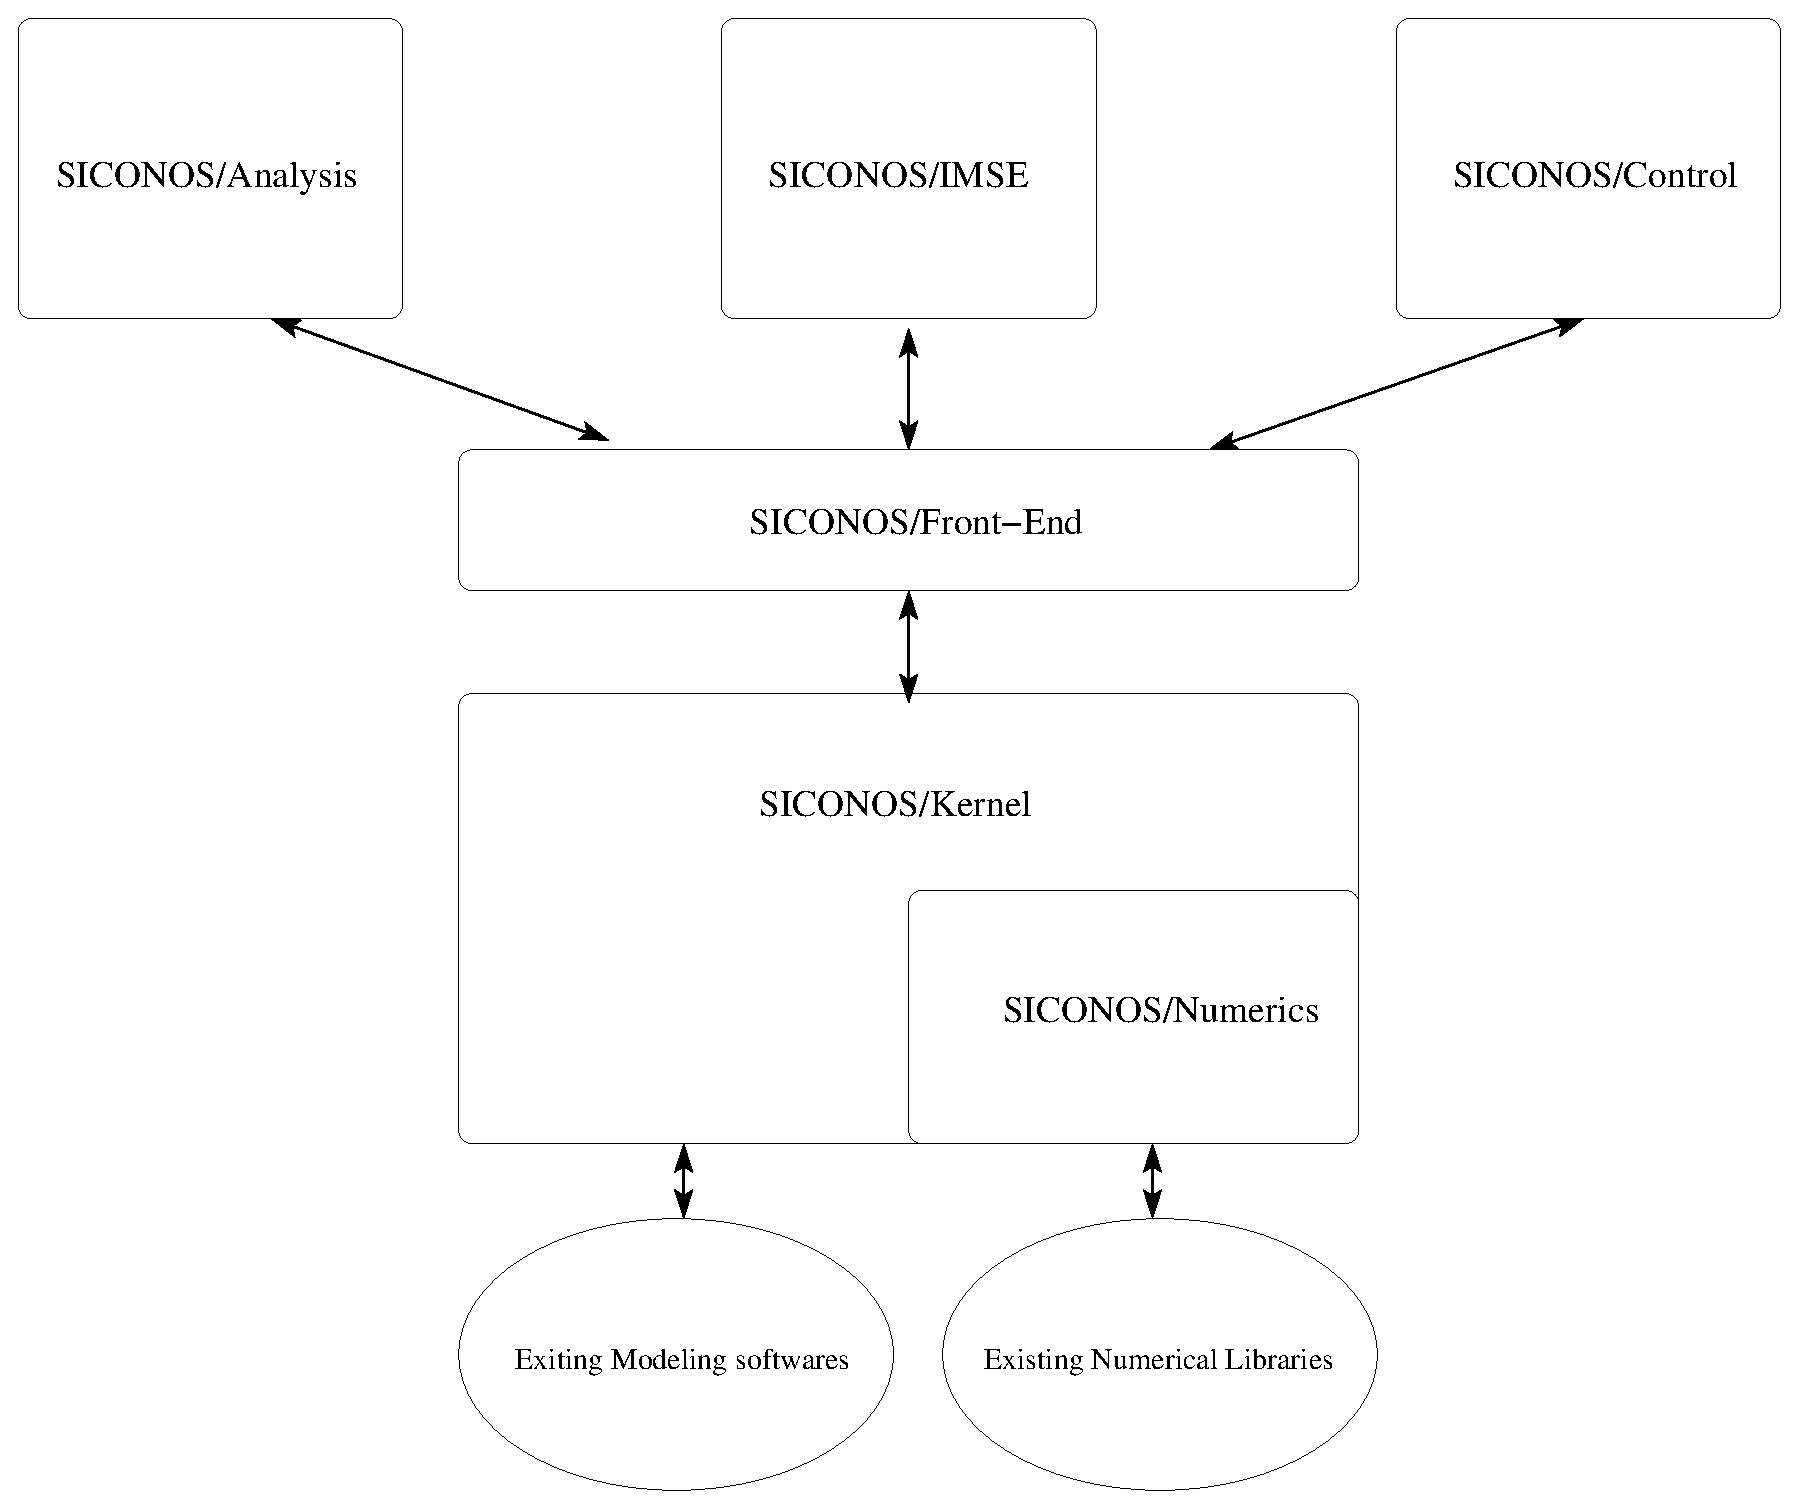
\includegraphics[width=0.7\textwidth]{./figure/functionalities.eps}
  \caption{Overview of the six functionalities of the \ac{siconos} Platform}
  \label{Fig:SICONOS-func}
\end{figure*}
\clearpage


\subsection{\acs{numerics}. Low-level numerical tools}
\label{Sec:SICONOS/Numerics}
This module will provide classes and methods to instantiate algebraic objects (vector, matrix, ...), 
with various storage formats (full, band, skyline ...). \\

This module has to perform various numerical functionalities~:
\begin{itemize}
 \item Linear algebra: linear system, eigenvalue, svd, ... \footnote{see LAPACK},
 \item Solver for non linear algebraic equation (Newton's method, ...),
 \item Solver for non smooth algebraic equation, (Generalized Newton Method, ...)
 \item Time integrator, ie basic computation for smooth time integration (one step integration, ...)
 \item Numerical, analytical or automatic differentiation,
 \item Mathematical programming (LCP, QP, optimization, ...).
\end{itemize}
%% \begin{ndrva}
%%   Doit on gerer les degres de liberte des integrateurs en temps dans Numerics ou dans Engine ? 
%% \end{ndrva}
\subsection{\acs{kernel}. Modelling and Simulation tools}
\label{Sec:SICONOS/Engine}



This module has to perform several major functionalities of the \ac{siconos} software. This module address  the modelling and the simulation  one physical process view as a non smooth dynamical system.


The functionalities of this module may be stated as follows:
\begin{enumerate}
\item \textbf{Model Formalization} :
  \begin{itemize}
  \item Define and describe several canonical model for general \ac{nsds}
    \begin{itemize}
    \item Linear complementarity systems (LCS)
    \item Lagrangian dynamical system with constraints
    \item Piecewise Smooth systems
    \item Higher order sweeping process
    \item Projected dynamical systems
    \item Unilateral differential inclusions
    \item Differential variational inequalities
    \item Discrete time system
    \end{itemize}
Several \ac{nsds} listed above (e.g LCS) may be decomposed in a smooth dynamical system, a set of relations between input/output variables and the state variables and a set of Non Smooth law which are listed below.
  \item Define and describe several canonical model for smooth dynamical systems SDS and the boundary conditions (IVP, BVP, ...)
    \begin{itemize}
    \item Linear Time invariant System (LTI)
    \item Non Linear System
    \item Lagrangian system
    \item Implicit System and differential Algebraic system
    \end{itemize}
  \item Define and describe several canonical model for relations between input/output variables and the state variables.
    \begin{itemize}
    \item Linear Time invariant relation
    \item Lagrangian relations (Jacobian)
    \item Non linear relations             \ldots
    \end{itemize}
  \item Define and describe several canonical model for non smooth Law
    \begin{itemize}
    \item Complementarity problem
    \item Relay system
    \item Friction-type law, etc.
    \end{itemize}
  \item Formalization of input systems into canonical model (general \ac{nsds}, SDS, Relations and non smooth laws)
  \item Analysis of coherence of the input systems 
  \item Translation between the  canonical models (general \ac{nsds}, SDS, and non smooth laws)
  \item Interface with description model tools (Plug-ins)(Existing modelling software, C F77 function, \ac{matlab} or \ac{scilab} function )
  \end{itemize}

\item  \textbf{Numerical strategies}
A numerical strategy is not only a set of basic numerical methods. It comprises the reformulation and the organization of the canonical model provided by the formalization part to realize the numerical computation. A numerical strategy is composed of :
  \begin{itemize}
  \item A time integrator method : Time--stepping or Event--Driven schemes.
  \item Evaluation or prediction of relations at discrete time. 
  \item Formalization of a one-step basic problem (LCP, QP, etc ...).
  \item Choice of a numerical method for solving the one step problem.   
  \item Interface with \ac{siconos}/numerics.
  \item Input/ Output of specific parameters for numerical strategies.
  \end{itemize}
\item  \textbf{Data representation and Save/Restart} The \ac{siconos} platform works with its own internal data structure, stored in the various attributes of the instantiated objects.  This internal data structure will consist of :
  \begin{itemize}
  \item data for the model formalization,
  \item data for the numerical strategy.
  \end{itemize}
Therefore, a specific storage structure  must be defined and constitutes the  \ac{siconos} specific files. This storage structure has to be very close to the object oriented data structure. The use of \ac{xml} and associated tools (DOM) seems  impossible to circumvent. 

If the \ac{siconos} specific files do not contain the complete representation of the formalized model, it needs to specify how to construct this representation, i.e. the name of the plug-in and the identifier of the data files for this plug-in.


Indeed, there are 3 ways to inform the internal data structure :
\begin{itemize}
\item The complete representation of the problem is loaded by reading \ac{siconos} specific and self-contained files. This way corresponds to a stand alone use of the platform.
\item The complete representation of the problem is loaded partially by reading \ac{siconos} specific files. In order to complete the missing part, the user has to provide the information using the API in interactive mode (object--oriented scripting language or the \ac{xxxlab} interface).
\item The complete representation of the problem is given by mixed files : external files describing the physical problem and its state and \ac{siconos} specific files describing the  model formalization and the numerical strategy. This way corresponds to a mixed use of the platform, in combination with an external software.
\end{itemize}

There are 2 ways to save the internal data structure :
\begin{itemize}
\item Using the \ac{siconos} specific and self-contained files,
\item Using mixed files: \ac{siconos} specific files and files saved by the external software.
\end{itemize}

Furthermore, the structure of the \ac{siconos} specific files must be able to represent all the above way to read and to save the data. It means that even for a mixed representation, the location of the external files must be specified in the \ac{siconos} specific files. 

Using these various mechanisms of reading and saving data, one can translate storage structure from external files to \ac{siconos} specific files.

This files must be exhaustive to allow a backup and a restart of a simulation at any specified time.  

The Engine must allow the user to trace internal variables during a simulation. These values of the internal variables could be exported in various formats for other post-processing softwares.

\end{enumerate}



%% \begin{ndrva}
%%   Mettre une figure de ce module. Tous les aspects pr�sents sur la figure doivent tre expliquer dans le texte.
%% \end{ndrva}

\subsection{\acs{frontend} }
\label{Sec:SICONOS/Front-End}

This module addresses the interface between the user and the platform. This interface have to fulfill several tasks :
\begin{itemize}
  \item To drive(command) the platform, i.e, to design a strategy of simulation,
  \item To provide an high-level language (logical tests, loops, \ldots),
  \item To be able to manage some basic mathematical computations,
  \item To provide informations to complete the data structure of the \ac{siconos}/Engine in interactive mode,
  \item To load external functions.
\end{itemize}


This Front-End will be realized by two APIs :
\begin{itemize}
\item A C++ API used through an object--oriented scripting language, 
\item An \ac{xxxlab} API used through \ac{xxxlab}. 
\end{itemize}




\subsection{\acs{control}.}
\label{Sec:SICONOS/Control}


The  major functionalities of the \ac{siconos}/Control  module are of the following :
\begin{itemize}
\item Validation of control strategies for \ac{nsds}
\item Feedback control with observers for \ac{nsds}
\item Trajectory planning     
\item Optimal control with constraints on the state and/or on the input.
\end{itemize}

In fact, the \ac{siconos}/Control  module will be built as an external module based on the C++ API provided by the \ac{siconos}/Front-end.

\subsection{\acs{analysis}.}
\label{Sec:SICONOS/Analysis}


This module  concerns the analysis of non smooth dynamical systems.  It provides several functionalities~:
\begin{itemize}
\item To check existence or well posed criteria, if any,
\item To search particular types of solutions (Periodic, steady-state, equilibrium sets,\ldots)
\item To study the stability of solutions (stable and unstable manifold.)
\item To perform  critical point detection (bifurcation detection)
\item To perform parametric continuation (path following methods)
\end{itemize}

Like the previous one, the \ac{siconos}/Analysis  module will be built as an external module based on the C++ API provided by the \ac{siconos}/Front-end.

\subsection{\acs{imse}.}
\label{Sec:SICONOS/pre-post}
 This module provides a  modelling and visualization environment for the \ac{kernel} based an the C++ API. Such a graphical  user interface  is  not planed, yet.

\section{General overview of the platform}

The platform should be used at three different levels~:
\begin{itemize}
\item in a partial level, using only the \ac{siconos}/Numerics part. It should be used in a standalone or interfaced through \ac{xxxlab},
\item in a global level through the standalone or the \ac{xxxlab} interface,
\item in a nested level through the \ac{siconos}/Control or \ac{siconos}/Analysis toolboxes.
\end{itemize}


\begin{sidewaysfigure}
  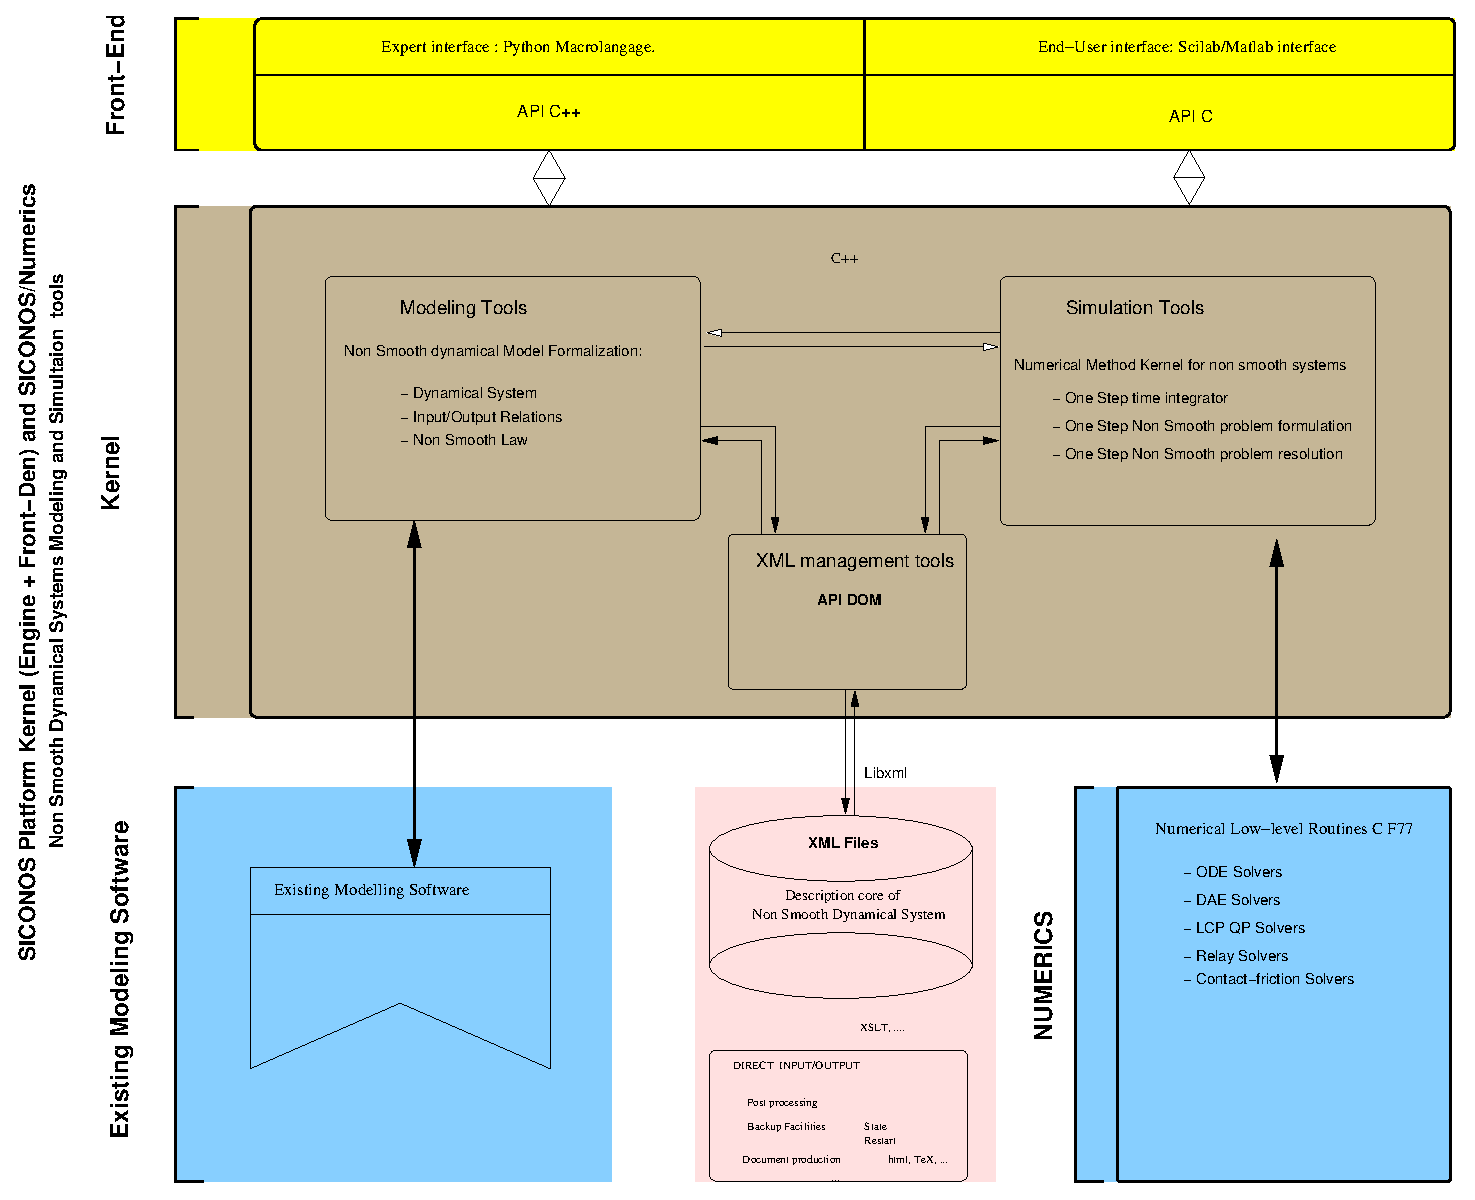
\includegraphics[width=0.8\textwidth]{./figure/Spec-v4.eps}
\end{sidewaysfigure}

\clearpage


%  use cases
\subsection{Users of the platform}

Three kind of users has been identified :
\begin{itemize}
\item End user : simplys uses the platform to run "basic"simulations.
\item Expert user : uses th platform to run simulations, but is also able to develop plugins with its own computation methods.
\item Developer : can add to the platform new features.
\end{itemize}.

%Diagramme d,utilisation general :
\begin{figure}[hb]
\begin{center}
\includegraphics[scale=0.65, bb=30 324 500 830, clip]{use_case_high_level.eps}
\end{center}
\caption{General use case}
\label{Fig:General use case}
\end{figure}

To get more details about the major features for each kind of users, see \ac{esd}.


%%%%%%%%%%%%%%%%%%%%%%%%%%%%%




\subsection{Flow-charts}

%\begin{ndrva}
%  Some flow charts will be interesting.  Goal: to fix ideas about the role of the modules and their relative independence.
%\end{ndrva}
The figure \ref{Fig:general_function} shows that it is possible to use external
application file (like \ac{lmgc90} file) via a dedicated plugin. An \ac{xml} plugin will
be provided to read \ac{xml} file.
The platform extracts some values from the simulation, and at the end of the
simulation, or at given steps of the simulation, the platform save the complet
state of the system in an \ac{xml} file. If we use this file as an input of the platform, we can restart the simulation at this point. 

\begin{figure}[hb]
\begin{center}
\includegraphics[angle=270, scale=0.85]{figure/GeneralFunctionning.eps}
\end{center}
\caption{General Functioning and files used}
\label{Fig:general_function}
\end{figure}
%%% Local Variables: 
%%% mode: latex
%%% TeX-master: "../report"
%%% End: 


%---------------------------------------------------------------------%
\newpage
\chapter{Specific requirements}
\label{Sec:SSD-SpecificRequirements}
%---------------------------------------------------------------------------%
%\section{Model and numerical methods related requirements}

%---------------------------------------------------------------------------%
\section{Functional requirements}
\label{Sec:SSD-FunctionalRequirements}
\subsection{\ac{siconos}/Numerics}
\begin{longtable}{%
    |>{\columncolor[gray]{.8}}p{0.1\textwidth}%
    |>{\columncolor[gray]{.95}}p{0.9\textwidth}|}
  \hline
  \rowcolor[gray]{.8}   SR. Id. & Software requirements description \\
  \hline 
  \hline
  & \textbf{General  requirements (\ac{siconos}/Numerics)}\\
  \hline 
  F.1.001 & The module \ac{siconos}/Numerics must provide basic algebra objects (vector, matrices, quaternions) relying on a matrix template library \\
  F.1.002 & The module \ac{siconos}/Numerics must provide  high performance methods for  basic vector and matrix operations\\
  F.1.003 & The module \ac{siconos}/Numerics must provide various storage methods for matrices:
  \begin{enumerate}
  \item Dense(full)
  \item Band
  \item Skyline
  \item Sparse
  \end{enumerate}\\
 \hline 
 & \textbf{ Numerical functionalities  requirements (\ac{siconos}/Numerics)}\\
  \hline
  F.1.010 & The module  \ac{siconos}/Numerics has to perform basic linear algebra computations  relying on standard libraries for numerical computation (e.g. LAPACK):
  \begin{enumerate}
  \item Solution of linear system 
  \item Eigenvalue and eigenvectors problem
  \item Singular Value Decomposition
  \end{enumerate}
  \\
  F.1.011 & The module \ac{siconos}/Numerics has to perform solution for mathematical programming problems:
  \begin{enumerate}
  \item Linear Complementarity Problem (LCP) (direct and iterative solutions) 
  \item Quadratic problem (QP) 
  \item Non Linear  Complementarity Problem (NCP) 
  \item General non smooth optimization problem
  \end{enumerate}\\
  F.1.012 & The module \ac{siconos}/Numerics has to perform basic computation for smooth time integration (one-step integration)  \\
  F.1.013 & The module \ac{siconos}/Numerics has to perform root finding for non linear smooth equations (Newton's method)\\
  F.1.014 & The module \ac{siconos}/Numerics has to perform root finding for non smooth (generalized) equations  \\
  F.1.015 & The module \ac{siconos}/Numerics has to perform numerical, analytical and automatic differentiation\\
  \hline

  & \textbf{Interface  requirements (\ac{siconos}/Numerics)}\\
  \hline 
   F.1.020 & The module \ac{siconos}/Numerics must provide a common interface to various methods dedicated to one specific type of numerical problem\\
  \hline
  \caption{\ac{siconos}/Engine. Software Requirements}\\
\end{longtable}



%-------------------------------------------------------------------------------------------------------------------------------%
\subsection{\ac{siconos}/Engine}
\begin{longtable}{%
    |>{\columncolor[gray]{.8}}p{0.1\textwidth}%
    |>{\columncolor[gray]{.95}}p{0.9\textwidth}|}
  \hline
  \rowcolor[gray]{.8}   SR. Id. & Software requirements description \\
  \hline 
  \hline
  & \textbf{ General requirements (\ac{siconos}/Engine)}\\
  \hline
  F.2.000 & The s/w shall propose a set of  canonical models to formalize physical process  (Model Formalization) \\
  F.2.001 & The s/w shall propose a set of numerical strategies to simulate the  canonical models (Numerical model)\\
  F.2.002 & The s/w  must be based on \ac{siconos}/Numerics  for the basic  scientific computation \\
  \hline
  & \textbf{Model Formalization requirements }\\
  \hline
  F.2.010  &  The s/w shall  define and describe several canonical model for general NSDS \\
  F.2.011  &  The s/w shall  define and describe several canonical model for SDS\\
  F.2.012  &  The s/w shall  define and describe several canonical model for relations\\
  F.2.013  &  The s/w shall  define and describe several canonical model for Non Smooth Laws\\  
  F.2.014  &  The s/w shall  define and describe a canonical model for LCS  \\
  F.2.015  &  The s/w shall  define and describe a canonical model for Lagrangian dynamical system with constraints \\
  F.2.016  &  The s/w shall  define and describe a canonical model for Piecewise Smooth systems \\ 
  F.2.017  &  The s/w shall  define and describe a canonical model for Higher order sweeping process\\ 
  F.2.018  &  The s/w shall  define and describe a canonical model for Projected dynamical systems \\ 
  F.2.019  &  The s/w shall  define and describe a canonical model for Unilateral differential inclusions \\
  F.2.020  &  The s/w shall  define and describe a canonical model for Differential variational inequalities  \\
  F.2.021  &  The s/w shall  define and describe a canonical model for Discrete time systems\\
  F.2.022  &  The s/w shall  define and describe a canonical model for Linear Time invariant System (LTI)\\ 
  F.2.023  &  The s/w shall  define and describe a canonical model for Non Linear System \\
  F.2.024  &  The s/w shall  define and describe a canonical model for Lagrangian system\\
  F.2.025  &  The s/w shall  define and describe a canonical model for Implicit System and differential Algebraic system\\
  F.2.026  &  The s/w shall  define and describe a canonical model for Linear Time invariant relation  \\  
  F.2.027  &  The s/w shall  define and describe a canonical model for Lagrangian relations (Jacobians)\\  
  F.2.028  &  The s/w shall  define and describe a canonical model for Non linear relations            \\  
  F.2.029  &  The s/w shall  define and describe a canonical model for Complementarity problem   \\  
  F.2.030  &  The s/w shall  define and describe a canonical model for Relay system              \\  
  F.2.031  &  The s/w shall  define and describe a canonical model for Friction-type law\\ 
  & \\
  F.2.040  &  The Model Formalization part must provide all of the ingredients for the numerical strategies part \\
  F.2.041  &  The model Formalization shall provide several  translation tools between the  canonical models if possible. (general NSDS, SDS, and non smooth laws) \\
  F.2.042  &   The s/w shall propose mechanisms to define the canonical model through C F77 functions. This is the Basic plug-in \\
  F.2.043  &   The s/w shall propose mechanisms (Plug-ins) to define the canonical model through 
  \begin{enumerate}
  \item \ac{matlab} functions 
  \item \ac{scilab} functions
  \end{enumerate}\\
  F.2.044  &   The s/w shall propose mechanisms (Plug-ins) to define the canonical model through Existing modelling software :
  \begin{enumerate}
  \item \ac{lmgc90} Plug-in
  \item \ac{modelica} Plug-in
  \item \ac{scicos} Plug-in
  \item \ac{simulink} Plug-in
  \end{enumerate} \\
  F.2.045  &   The s/w shall propose several tools for the analysis of the coherence of the  input\\
 \hline
  & \textbf{Numerical strategies requirements }\\
  \hline
  F.2.100  & The s/w shall propose a Time--stepping scheme\\
  F.2.101  & The s/w shall propose a Event--Driven scheme\\
  F.2.102  & The s/w shall propose a formalization of a one-step basic problem\\
  F.2.103  & The s/w shall propose an evaluation or prediction of the relations at discrete time\\
  F.2.104  & The s/w shall propose an input method for specific parameters for numerical strategies\\
  F.2.105  & The s/w shall propose an output method for specific parameters for numerical strategies\\
  \hline
  & \textbf{Interface with \ac{siconos}/Numerics }\\
  \hline
  F.2.200  & The module \ac{siconos}/Engine must use the interface proposed by the  \ac{siconos}/Numerics module for the numerical computations \\
  \hline
  & \textbf{Data managing}\\
  \hline
  F.2.300  &  The software must be able to call functions of exiting scientific softwares to read their own data files. Only \ac{lmgc90} files will be called in the first version of the plate-forme. \\
  F.2.301  & The software must allow users to save a NSDS in files under a formalized form. \\
  F.2.302  & The software must be able to proceed to several files formats conversions.
                \begin{enumerate}
                \item \ac{lmgc90} file to XML file.
                \item XML file to external software file (GNUplot).
                \end{enumerate}\\ 
  F.2.303  & The software must allow users to trace states of a modelised system during a simulation. \\
  F.2.304  & The software must provide a system of backup and restart of a simulation, using XML files. \\
  \caption{\ac{siconos}/Engine. Software Requirements}\\
\end{longtable}



%-------------------------------------------------------------------------------------------------------------------------------%
\subsection{\ac{siconos}/Front-End}
\begin{longtable}{%
|>{\columncolor[gray]{.8}}p{0.1\textwidth}%
|>{\columncolor[gray]{.95}}p{0.9\textwidth}|}
\hline
\rowcolor[gray]{.8}   SR. Id. & Software requirements description \\
\hline 
   & \textbf{ General requirements (SICONOS/Front-End)}\\
   \hline
   F.3.000 & The \ac{siconos}/Front-End shall propose a C++  API  of the major functionalities of the \ac{siconos}/Engine (Functionalities F.2.xxx)  . In particular, this API will be wrapped to a object--oriented scripting language). \\
   F.3.001 & The \ac{siconos}/Front-End shall propose a \ac{scilab}  API  of the major functionalities of the \ac{siconos}/Engine (Functionalities F.2.xxx)  . In particular, this API will be  called trough the \ac{scilab} software. \\ 
   F.3.002 & The \ac{siconos}/Front-End shall propose a \ac{matlab}  API  of the major functionalities of the \ac{siconos}/Engine (Functionalities F.2.xxx)  . In particular, this API will be  called trough the \ac{matlab} software. \\
   F.3.003 & The \ac{siconos}/Front-End shall propose a C++  API well-suited (completeness and granularity) for the the analysis (\ac{siconos}/Analysis), the control (\ac{siconos}/Control).    \\
\hline
\caption{\ac{siconos}/Front-End. Software Requirements}\\
\end{longtable}
\subsection{SICONOS/Control.}

The specific requirements for the \ac{siconos}/Control will be defined later. 
\begin{longtable}{%
|>{\columncolor[gray]{.8}}p{0.1\textwidth}%
|>{\columncolor[gray]{.95}}p{0.9\textwidth}|}
\hline
\rowcolor[gray]{.8}   SR. Id. & Software requirements description \\
\hline 
   & \textbf{ General requirements (\ac{siconos}/Control.)}\\
   \hline
   F.4.000 & \\
\hline
\caption{\ac{siconos}/Control. Software Requirements}\\
\end{longtable}
\subsection{\ac{siconos}/Analysis.}

The specific requirements for the \ac{siconos}/Analysis will be defined later.
\begin{longtable}{%
|>{\columncolor[gray]{.8}}p{0.1\textwidth}%
|>{\columncolor[gray]{.95}}p{0.9\textwidth}|}
\hline
\rowcolor[gray]{.8}   SR. Id. & Software requirements description \\
\hline 
   & \textbf{ General requirements (\ac{siconos}/Analysis.)}\\
   \hline
   F.5.000 & \\
\hline
\caption{\ac{siconos}/Analysis. Software Requirements}\\
\end{longtable}
\subsection{\ac{siconos}/IMSE.}
The specific requirements for the \ac{siconos}/IMSE will be defined later.

\begin{longtable}{%
|>{\columncolor[gray]{.8}}p{0.1\textwidth}%
|>{\columncolor[gray]{.95}}p{0.9\textwidth}|}
\hline
\rowcolor[gray]{.8}   SR. Id. & Software requirements description \\
\hline 
   & \textbf{ General requirements (\ac{siconos}/IMSE.)}\\
   \hline
   F.6.000 & \\
\hline
\caption{\ac{siconos}/IMSE. Software Requirements}\\
\end{longtable}



 
%%% Local Variables: 
%%% mode: latex
%%% TeX-master: "../report"
%%% End: 



%---------------------------------------------------------------------------%

\section{Performance requirements}
\begin{longtable}{%
|>{\columncolor[gray]{.8}}p{0.1\textwidth}%
|>{\columncolor[gray]{.95}}p{0.9\textwidth}|}
   \hline
\rowcolor[gray]{.8}   SR. Id. & Software requirements description \\
      \hline 
   & \textbf{ Performance requirements }\\
   \hline
   PER.00 & The software mustn't be more than 10\% slower than \ac{lmgc90} for the same treatement on the same computer. \\
\hline
\caption{Performance Requirements}\
\end{longtable}

%---------------------------------------------------------------------------%
%\section{Data representation requirements}


%\begin{longtable}{% |>{\columncolor[gray]{.8}}p{0.1\textwidth}% |>{\columncolor[gray]{.95}}p{0.9\textwidth}|}
%\hline
%\rowcolor[gray]{.8}   SR. Id. & Software requirements description \\
%   \hline 
%   & \textbf{Data representation }\\
%   \hline
%   DAT.00 & Files representing formalized \ac{nsds} and generated by the s/w will be \ac{xml} files. \\  
%\hline
%\caption{Data representation requirements}
%\end{longtable}
%---------------------------------------------------------------------------%


%---------------------------------------------------------------------------%
\section{Interface requirements and Users environments related requirements}
\begin{longtable}{%
    |>{\columncolor[gray]{.8}}p{0.1\textwidth}%
    |>{\columncolor[gray]{.95}}p{0.9\textwidth}|}
  \hline
  \rowcolor[gray]{.8}   SR. Id. & Software requirements description \\
  \hline 
  & \textbf{Users interfaces requirements }\\
  \hline
  INT.00 & The software should provide an API. \\
  INT.01 & This API can be used by a C++ software.\\
  \hline 
%  & \textbf{Interfaces requirements with Existing modelling software }\\ 
%  \hline
%  INT.10 & High-level functions of the software must be usable through \ac{scilab}.  \\
%  INT.11 & High-level functions of the software must be usable through \ac{matlab}.  \\
%  \hline
  \caption{Interface requirements}\\
\end{longtable}


Discuss the use conditions (user-friendly, accessibility, \ldots) and the level of abstraction for different classes of users :
\begin{itemize}
%\item frameworks builders
%\item Component builders
\item Algorithm developers
\item End users
\end{itemize}

%---------------------------------------------------------------------------%
\section{Resource requirements}
\begin{longtable}{%
|>{\columncolor[gray]{.8}}p{0.1\textwidth}%
|>{\columncolor[gray]{.95}}p{0.9\textwidth}|}
   \hline
\rowcolor[gray]{.8}   SR. Id. & Software requirements description \\
      \hline 
   & \textbf{Resource requirements }\\
   \hline
   RES.00 &  This configuration is recommended : processor 800 MHz, 512 Mo Ram, 20 Mo of free space on HDD.\\
\hline
\caption{Resource requirements}
\end{longtable}
%---------------------------------------------------------------------------%

\section{Documentation requirements}
\begin{longtable}{%
    |>{\columncolor[gray]{.8}}p{0.1\textwidth}%
    |>{\columncolor[gray]{.95}}p{0.9\textwidth}|}
  \hline
  \rowcolor[gray]{.8}   SR. Id. & Software requirements description \\
  \hline 
  & \textbf{ Documentation type requirements }\\
  \hline
  DOC.1.00 & The documentation must contain a Software User Manual (SUM)  \\
  DOC.1.01 & The documentation must contain a Tutorial Manual\\
  DOC.1.02 & The documentation must contain a Example problems Manual\\
  DOC.1.03 & The documentation must contain a Benchmarks \& Verification Manual\\
  DOC.1.04 & The documentation must contain a Theory Manual\\
  DOC.1.05 & The documentation must contain a Interface users Manual\\
  DOC.1.06 & The documentation must contain a Developer Manual\\
  \hline 
  & \textbf{ Documentation format requirements }\\
  \hline
  DOC.2.00 & The source of the various manual must be in TeX format\\
  DOC.2.01 & The various manual must be available in HTML format\\
  DOC.2.02 & The various manual must be available in PDF format\\
  DOC.2.03 & The various manual must be written in English.\\
 \hline
  \caption{Documentation requirements}\\
\end{longtable}



%---------------------------------------------------------------------------%
\section{Portability requirements}
\begin{longtable}{%
|>{\columncolor[gray]{.8}}p{0.1\textwidth}%
|>{\columncolor[gray]{.95}}p{0.9\textwidth}|}
   \hline
\rowcolor[gray]{.8}   SR. Id. & Software requirements description \\
      \hline 
   & \textbf{  Hardware and Operating system support }\\
   \hline
   POR.1.00 & The s/w must run on PC/Linux environment \textit{kernel 2.4.20-8}\\
   POR.1.01 & The s/w must run on PC/Windows environment \textit{Microsoft Windows 2000}\\
   POR.1.02 & The s/w must run on Sun Workstation/Sun OS-Solaris environment \textit{Solaris 5.8}\\
   POR.1.03 & The s/w must run on  Apple/Mac OS X environment \\
   \hline 
   & \textbf{ Data portability}\\
   \hline
   POR.2.00 & The ASCII data files must be portable (specify an unique charset)\\ 
   POR.2.01 & The BINARY data files must be portable (specify a binary format,IEEE norm)\\ 
   \hline
\caption{Portability requirements}\\
\end{longtable}

%---------------------------------------------------------------------------%
%\section{Quality requirements}

%After an analysis of \ac{siconos} software requirements, four priority software quality factors (Mc Call criteria) have been chosen. Each one has a mark of priority.
%\begin{longtable}{%
%|>{\columncolor[gray]{.8}}p{0.1\textwidth}%
%|>{\columncolor[gray]{.95}}p{0.9\textwidth}|}
%   \hline
%\rowcolor[gray]{.8}   SR. Id. & Software requirements description \\
%      \hline 
%   & \textbf{ Quality requirements }\\
%   \hline
%   QUA.00 & Adaptability (or flexibility). \textit{9/10}\\
%   QUA.01 & Efficiency.\textit{8/10}\\
%   QUA.02 & Couplability. \textit{7/10}\\ 
%   QUA.03 & Portability. \textit{5/10}\\
%   \hline
%\caption{ Quality requirements}\\
%\hline
%\end{longtable}

%Here are short definitions of those criteria and the reasons why they were chosen as priority quality factors for this project.

%\begin{itemize}
%\item   Adaptability : \\
%        It measures the ability of the software to make easier additions of new functionalities or modifications, even suppression of existing functionalities. This factor has been chosen because users must be able to add easily new algorithms or computations libraries. 
%\item   Efficiency : \\
%        It measures the ability of the software to minimize its resources needs (cpu time, memory, etc.).
%        This criterion is necessary for a scientific computation software.
%\item   couplability : \\
%        Capacity of the software to be used with other softwares (data exchanges, calls, ...).
%        Like the plateforme can be accessible via \ac{scilab}, this factor is important.
%\item   Portability : \\
%        Capacity of the software to reduce consequences of an environment technical change (hardware or software).
%        Users come from several laboratories and companies, and work under several OS.
%\end{itemize}





%---------------------------------------------------------------------%
\newpage
\chapter{System Overview}
\label{Sec:SSD-SystemOverview}
%\begin{ndr}
%  This section should briefly introduced  to the system context and design. The section may summarise the costs and benefits of the selected architecture, and may refer to prototyping exercises.
%\end{ndr}


\section{Context and design of the system}

The \ac{siconos} will be used to simulate several classes of Non Smooth Dynamical Systems
\acs{nsds} (see \ac{um}).\\

The platform will be written in C++ and used as a library. It's planned to be used through a
C++ program which can be compiled or interpreted, or through an external computation software (\ac{xxxlab}). For more details, we refer to the \ac{esd}\\

The software may be decomposed in three parts~:
  \begin{itemize}
        \item \acs{numerics} for numerical computations~;
        it contains routines for low level operations. 
        \item \acs{engine} for high level description and numerical solving strategies of \ac{nsds};
        it represents the core of the platform, that is to say the knowledge of the software. It is there that the end user will find (the expert user will add) models and algorithms to simulate \ac{nsds}. The  numerical part of the  \acs{engine} relies on \acs{numerics} routines. Indeed, the Engine  drives modelisation, simulation, input/output and plug-ins modules.
        \item \acs{frontend} is the only part of the software which will be accessible by end
	users and all the other users. It allows to use the functions of the Engine.
  \end{itemize}
  
  
\section{Costs and benefits of the architecture}
The choice of the software design will have a cost for the overall performances in comparison to the original software written in Fortran
(\ac{lmgc90} which is dedicated to mechanical problems). However, the loss of performance won't be so important because all the time consuming computations will be performed with optimised Fortran or C routines.
  
Otherwise the architecture will improve the flexibility and the couplability of the software. So the platform will be evolutionary.


\section{Prototyping exercises}
Some points must be evaluated so it will be useful to develop prototypes. For the following items, we will make prototypes~:
\begin{itemize}
        \item libXML prototype, to manipulate \ac{xml}~;
        \item The plug-ins prototype, for input extensions~;
        \item C++ interpreter prototype, which uses a library~;
\end{itemize}

With all these prototypes, another one will be built, regrouping these one. It will be in other words a prototype to see if the
tools we will use can work together, a prototype to see the integration of the different modules.

%---------------------------------------------------------------------%
\newpage
\chapter{Conceptual System Design}
\label{Sec:SSD-ConceptualSystemDesign}
\section{Analysis}
\ac{numerics} has to be a library regrouping other libraries. Each one corresponds to a part of the source of \ac{numerics} and is composed of source files in C or Fortran.\\
The architecture that suites is a set of directories to arrange all the libraries.\\
Into each directory according to a specific library, whereas programming languages are non object oriented, every file regroups functions relating to a particular kind of operation or system.


\section{Decomposition description}
The software components should be summarised. These components can be organised in various ways to provide the
views needed by the different members of the development team. The following views present the software
design.

\subsection{Decomposition view}
Here, we show the functional decomposition of the components. It consists in a list of components summarised~:
 
\begin{itemize}
		\item \ac{lapack}\\
		It is routines for solving systems of simultaneous linear equations, least-squares solutions of linear systems of equations, eigenvalue problems, and singular value problems.

        \item MP solver pack\\
		It regroups all the functionalities to solve non-smooth problems.
		
        \item \ac{ode} pack\\
		It is a collection of Fortran solvers for the initial value problem for ordinary differential equation systems.

        \item ...\\
\end{itemize}


\subsection{Dependency view}
Each module of \ac{numerics} is independent from the others. They make different kinds of computations and each module regroups specific low level functions.
However, \ac{lapack} is commonly used by the other "packs" (MP solver pack, \ac{ode} pack, \dots). It is the basis for the operations of these "packs".


\section{System architecture diagram with related description}
The figure \ref{fig: Tree view of the Numerics directories} represents the architecture of \ac{numerics}'s directories.
	\begin{figure}
	\begin{center}
	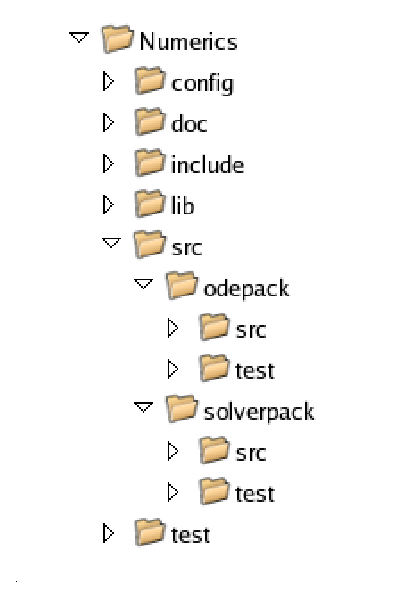
\includegraphics[scale=1.2, clip]{figure/NumericsDesign.eps}
	\caption{Tree view of the Numerics directories}
	\label{fig: Tree view of the Numerics directories}
	\end{center}
	\end{figure}
	
Each \textit{src} directory contains the source code of \ac{numerics}, especially \textit{src/odepack/src} and \textit{src/solverpack/src} which contain the code of \ac{ode} pack and MP solverpack.

%---------------------------------------------------------------------%
\newpage
\chapter{Component Description}
\label{Sec:SSD-ComponentDescription}
\section{Front-End Package}

	The class diagram \ref{fig: Class diagram for the front-end} shows the structure we will use for this package.
	
	\begin{figure}
	\begin{center}
	\includegraphics[bb=25 720 300 830, clip]{figure/class_frontend.ps}%35 540 560 830
	\caption{Class diagram for the front-end}
	\label{fig: Class diagram for the front-end}
	\end{center}
	\end{figure}
	


	\subsection{Component ``enter choice''}
		
		\begin{description}
	
		\item[Identifier~:]EnterChoice
		\item[Type~:]Method
		\item[Function-processing~:]Offer to read data or to run the simulation for the user. Transmits the result to the ``connect'' component.
		\item[Dependencies~:]-
		\item[Interfaces~:]Output : formalisation or simulation
		\item[Data~:]-

		\end{description}
	
	
  	\subsection{Component ``connect depending on choice''}
	
		\begin{description}
	
		\item[Identifier~:]Connect
		\item[Type~:]Method
		\item[Function-processing~:]Launch the read of the data or launch the simulation depending on the choice enter in the ``enterChoice'' component.
		\item[Dependencies~:]The component  ``enterChoice'' must be executed before this component is called.
		\item[Interfaces~:]Take as input the result of ``enterChoice''.
		\item[Data~:]-

		\end{description}

%  	\subsection{Component ``process manually input data''}
%	\begin{description}
%	\item[Identifier~:]ProcessManData
%	\item[Type~:]Module
%	\item[Function-processing~:]Process the data that are entered manually %using the interface. The data entered by the user (generally matrix
%	and function) are converted to a specified format in order to be %transmitted to the model formalisation package.
%	\item[Dependencies~:]The package  ``model formalisation'' must be %executed after this component is called.
%	\item[Interfaces~:]Take as input the data entered by the user.
%	\item[Data~:]-
%	\end{description}
	

	
\section{Model Formalisation Package}
	The class diagram \ref{fig: Class diagram for model formalisation} shows the structure we will use for this package.
	
	\begin{figure}
	\begin{center}
	\includegraphics[scale=0.85, bb=20 500 560 830, clip]{figure/class_formalisation.ps}
	\caption{Class diagram for model formalisation}
	\label{fig: Class diagram for model formalisation}
	\end{center}
	\end{figure}


	\subsection{Component ``fill dynamic system''}	
	
		\begin{description}
	
		\item[Identifier~:]FillDS
		\item[Type~:]Module
		\item[Function-processing~:]Fill the dynamic system part of the \ac{nsds}.
		\item[Dependencies~:]This component can be executed before, after or meanwhile the processing of the ``fill relations'' and the ``fill non smooth law'' component.
		\item[Interfaces~:]Take as input the data given by the Input/Output/Plug-in package. The output is the representation of the dynamic system.
		\item[Data~:]An inherited class of the DynamicSystem class.

		\end{description}
  	
	
	\subsection{Component ``fill relations''}
	
		\begin{description}
	
		\item[Identifier~:]FillRelations
		\item[Type~:]Module
		\item[Function-processing~:]Fill the relation part of the \ac{nsds}.
		\item[Dependencies~:]This component can be executed before, after or meanwhile the processing of the ``fill dynamic system'' and the ``fill non smooth law'' component.
		\item[Interfaces~:]Take as input the data given by the Input/Output/Plug-in package. The output is the representation of the relation.
		\item[Data~:]An inherited class of the Relations class.

		\end{description}
	
	
  	\subsection{Component ``fill non smooth laws''}
	
		\begin{description}
	
		\item[Identifier~:]FillNSLaw
		\item[Type~:]Module
		\item[Function-processing~:]Fill the non smooth laws part of the \ac{nsds}.
		\item[Dependencies~:]This component can be executed before, after or meanwhile the processing of the ``fill dynamic system'' and the ``fill relations'' component.
		\item[Interfaces~:]Take as input the data given by the Input/Output/Plug-in package. The output is the representation of the non smooth law.
		\item[Data~:]An inherited class of the NonSmoothLaw class.

		\end{description}

	
  	\subsection{Component ``update state''} \label{update_state}
	
		\begin{description}
	
		\item[Identifier~:]UpdateState
		\item[Type~:]Module
		\item[Function-processing~:]Update the state of the system when the model is formalised.
		\item[Dependencies~:]This component can be executed after the processing of the ``fill dynamic system'', ``fill relations'' and the ``fill non smooth law'' component, or after the ``computation'' execution (cf. section \ref{computations}).
		\item[Interfaces~:]Take as input data from the formalised model and save the system state with this data.
		\item[Data~:]System state

		\end{description}
	

\section{Numerical Strategy Package}

	The Class diagram \ref{fig: Class diagram for numerical strategy} shows the structure we will use for this package.
	
	\begin{figure}
	\begin{center}
	\includegraphics[bb=25 690 245 830, clip]{figure/class_numerical_strategy.ps}
	\caption{Class diagram for numerical strategy}
	\label{fig: Class diagram for numerical strategy}
	\end{center}
	\end{figure}
	
	


  	\subsection{Component ``increase time step''}
	
		\begin{description}
	
		\item[Identifier~:]IncreaseTimeStep
		\item[Type~:]Method
		\item[Function-processing~:]Give the signal for begin to simulate one time step
		\item[Dependencies~:]Its execution takes place before the ``predict interaction'' component execution
		\item[Interfaces~:]-
		\item[Data~:]-

		\end{description}
	
	
  	\subsection{Component ``predict interaction''}
	
		\begin{description}
	
		\item[Identifier~:]PredictInteraction
		\item[Type~:]Module
		\item[Function-processing~:]Predict the interaction between object.
		\item[Dependencies~:]This component can be executed only after ``increase time step''. It had to be executed before the ``verify constraint'' execution.
		\item[Interfaces~:]This component can use some functions defined in a specific plug-in. It uses the data stored in the system state to predict the interaction. 
		\item[Data~:]-

		\end{description}
	
  	\subsection{Component ``verify constraints''}
	
		\begin{description}
		
		\item[Identifier~:]VerifConstraints
		\item[Type~:]Module
		\item[Function-processing~:]Verify the constraint of the system (if 2 objects are not at the same place)
		\item[Dependencies~:]The component ``predict interaction'' must be executed before this component is called and ``make coherent'' 
		\item[Interfaces~:]This component can use some functions defined in a specific plug-in. It uses the data stored in the system state and the prediction of the interaction to verify the constraint.
		\item[Data~:]-

		\end{description}
	
  	\subsection{Component ``make coherent''}
	
		\begin{description}
	
		\item[Identifier~:]MakeCoherent
		\item[Type~:]Module
		\item[Function-processing~:]Make the system coherent if not
		\item[Dependencies~:]This component must be executed after ``verify constraint'' only if there is a constraint violation.
		\item[Interfaces~:]This component can use some functions defined in a specific plug-in. It uses the data stored in the system state and the data produced by the component ``verify the constraint'' to make the system coherent.
		\item[Data~:]-

	\end{description}
	
  	\subsection{Component ``computations''}\label{computations}
	
		\begin{description}
	
		\item[Identifier~:]Compute
		\item[Type~:]Module
		\item[Function-processing~:]Compute one time step using numerical libraries.
		\item[Dependencies~:]This component must be executed after ``verify constraint'' if there is non constraint violation and after ``make coherent'' in the other case.
		\item[Interfaces~:]This component can use some functions defined in a specific plug-in. It uses the data stored in the system state.
		\item[Data~:]-

		\end{description}
	
	\subsection{Component ``update state''} 
	cf. \ref{update_state}\\
	
	

\section{Input/Output/Plug-in Package}
	The Class diagram \ref{fig: Class diagram for specific plug-ins} shows the structure we will use for this package.
	
	\begin{figure}
	\begin{center}
	\includegraphics[bb=20 700 160 820, clip]{figure/class_specific_plugins.ps}
	\caption{Class diagram for specific plug-ins}
	\label{fig: Class diagram for specific plug-ins}
	\end{center}
	\end{figure}
	
	
  	\subsection{Component ``read \acs{xml} file''}
	
		\begin{description}
	
		\item[Identifier~:]ReadXML
		\item[Type~:]Module
		\item[Function-processing~:]Read the \ac{xml} file which describes the system state and the numerical strategy.
		\item[Dependencies~:]-
		\item[Interfaces~:]Take as input an \ac{xml} file and give in return the data and function describing the system.
		\item[Data~:]-

		\end{description}
	
  	\subsection{Component ``read and convert dedicated file''}
	
		\begin{description}
	
		\item[Identifier~:]ReadFile
		\item[Type~:]Module
		\item[Function-processing~:]Read and convert a dedicated file in order to have a description of the system state and the numerical strategy.
		\item[Dependencies~:]-
		\item[Interfaces~:]Take as input a specific file and give in return the data and function describing the system.
		\item[Data~:]-

		\end{description}
	
  	\subsection{Component ``bring out complete result''}
	
		\begin{description}
	
		\item[Identifier~:]CompletRes
		\item[Type~:]Module
		\item[Function-processing~:]Put the complete results in a \ac{xml} file
		\item[Dependencies~:]The computation of one time step must be finished.
		\item[Interfaces~:]Take as input the result of the component ``computation''.
		\item[Data~:]-

		\end{description}
	
  	\subsection{Component ``bring out partial result''}
	
		\begin{description}
	
		\item[Identifier~:]PartialResult
		\item[Type~:]Module
		\item[Function-processing~:]Put piece of results in a \ac{xml} file
		\item[Dependencies~:]The computation of one time step must be finished.
		\item[Interfaces~:]Take as input the result of the component ``computation''.
		\item[Data~:]-

		\end{description}



%---------------------------------------------------------------------%
\newpage
\printglosstex(acr)[p]

%===================================

\listoffigures
\listoftables
\cleardoublepage
%\bibliographystyle{plainnat}
%\bibliography{./Biblio/String,./Biblio/Cp.bib,./Biblio/Optim.bib,./Biblio/Contact.bib,./Biblio/NonSmooth.bib,./Biblio/Leger.bib,./Biblio/Petri.bib}
\cleardoublepage
\end{document}
